\chapter{\codet{pycapacity}: an efficient task-space capacity calculation Python package for robotics and biomechanics}
\label{ch:software}

Preceding chapters have demonstrated the potential of real-time evaluation of robot's and human's physical abilities for creating more flexible human-robot collaboration. \Cref{ch:physical_interaction} showed that the real-time evaluation of robot's and human's physical ability polytopes can be a valuable tool for creating adaptable robot control strategies for human-robot physical collaboration scenarios, able to adapt to their changing physical abilities.  \Cref{ch:informaiton_polytopes} discussed the potential of polytopes as a visual feedback tools for improving human operators' situational awareness, by providing them with real-time insight into the robot's current state and its changing abilities. Finally, \Cref{ch:topca} showed how real-time evaluation of robot's movement capacity enables creating more flexible trajectory planning strategies able to adapt to its changing physical abilities on the fly. 

However, all the described approaches heavily rely on the efficient evaluation of different physical ability polytopes, requiring their 
real-time their execution. As described more in detail in \Cref{ch:transformin_polytopes}, the computation complexity of polytope evaluation depends highly on its formulation and makes choosing the appropriate algorithm a crucial challenge when it comes to building such applications. 

Therefore, this chapter presents the software package called \codet{pycapacity}, which aims to provide a set of efficient tools for evaluating task-space physical ability metrics for humans and robots, based on polytopes and ellipsoids. The package implements several state-of-the-art algorithms for polytope evaluation, including VEPOLI$^2$ and ICHM developed in the context of this thesis and introduced in \Cref{sec:algorithm_vea} and \Cref{ch:algorihtm_ichm} respectively. In that way, it bringing many of the physical ability polytopes to the few milliseconds evaluation time, making it possible to use them in online and interactive applications. 

Furthermore, \codet{pycapacity} is implemented as a Python package with a goal to be an easy-to-use framework that can be easily integrated with standard robotics and biomechanics libraries. The package can be easily interfaced with standard libraries for robotic manipulator rigid body simulation such as \codet{roboticstoolbox} \cite{rtb} or \codet{pinocchio} \cite{pinocchio2021}, as well as human musculoskeletal model biomechanics software \codet{opensim} \cite{opensim} and \codet{biorbd} \cite{Michaud2021}. The package can also be used with the \gls{ros} \cite{ros}.

The package additionally implements a set of visualisation tools for polytopes and ellipsoids based on the Python package \codet{matplotlib} intended for fast prototyping and quick and interactive visualisation.

\Cref{sec:pycpacity_motivation} brings more detailed motivation behind the development of this package. \Cref{sec:pycapacity_ellip_poly} then brings a brief introduction in the differences between ellipsoids and polytopes and their evaluation within the package. \Cref{sec:pycapacity_robot} and \Cref{sec:pycapacity_human} list the implemented physical ability ellipsoids and polytopes. \Cref{sec:pycapacity_impelmented_polytopes} lists the implemented polytope transformation algorithms, followed by \Cref{sec:pycapacity_performance} which brings the performance analysis of the implemented polytope algorithms for different physical ability polytopes. Finally, \Cref{sec:pycapacity_package_overview} introduces the brief overview of the software implementation of the package and an example code.

\section{Motivation}
\label{sec:pycpacity_motivation}
% There is a rising interest in collaborative robotics and physical human robot interaction, where the robots are often required to adapt to certain needs of the human in real-time. This adaptation raises a fundamental challenge: the ability to evaluate the need of assistance of the operator. One way to quantify the need of assistance is by evaluating the operator's physical abilities in real-time and comparing them to the physical abilities required to execute the task. Having this real-time information enables creating collaborative robot control strategies that assist the operators by compensating for their lacking physical ability to accomplish the tasks.

% Beyond the characterization of human physical capabilities, as today's collaborative robotic manipulators are designed for safety, their performance characteristics are relatively limited with respect to the more standard industrial robots. Therefore it is becoming increasingly important to exploit their full (physical) abilities when executing their task.  

There are many different metrics available in the literature that might be used to characterise different physical abilities of humans and robots: force capacity, velocity capacity, acceleration capacity, accuracy, stiffness etc. Most of these metrics can be represented by two families of geometric shapes: ellipsoids \cite{yoshikawa1985manipulability} and polytopes \cite{chiacchio_evaluation_1996}. These metrics are traditionally important tools for off-line analysis purposes (workspace design, human motion and ergonomics analysis) and recently, they have shown a great potential to be used for interactive online applications, to be integrated in robot control strategies or as a visual feedback to the operator. 

Ellipsoid metrics are often used for evaluating the manipulability of the robot's end-effector. The manipulability ellipsoid is a geometric shape that represents the robot's ability to move within the task-space. Due to their computational efficiency and intuitive visualisation, they have been used in many different applications, such as robot control, workspace design, robot design, etc. Therefore, there are several 
open-source packages that implement the manipulability ellipsoid evaluation and visualisation, such as \codet{MMC} \cite{Haviland2020Maximising}, \codet{manipulability\_metrics} \cite{manipulability_metrics}, \codet{Manipulability} \cite{manipulability}\cite{Jaquier2021Geometry}. However, most of these packages are limited to the evaluation of the manipulability ellipsoid, representing the velocity capacity, and they do not provide tools for evaluating other ellipsoid metrics, such 
as force capacity, acceleration capacity, etc. Additionally these software packages are often developed for the use with a specific robotics library, such as \codet{roboticstoolbox} \cite{rtb} or \gls{ros} \cite{ros}, and they are not trivial to integrate with other libraries.

Even though different efficient tools for evaluating ellipsoids are widely available in the literature and open-source community, the tools for evaluating polytopes are still relatively scarce. The main reason for this is that the polytopes are in general more complex to evaluate and manipulate than ellipsoids. However, the polytopes are much more accurate representation of the true limits. Additionally, polytopes are easy to visualize, as they are essentially triangulated meshes, and they can be easily integrated in the robot control strategies, as they can be expressed as a set of linear constraints. 

The evaluation of polytopes is often a computationally expensive task, as their resolution requires using different vertex and facet enumeration algorithms \cite{fukuda2004frequently}. Therefore, their computation time is often the limiting factor for the use of polytopes in real world applications, especially when it comes to their online use. Furthermore, even though there are several open-source projects that implement polytope evaluation algorithms, such as \codet{pypoman} \cite{pypoman}, Multi-Parametric Toolbox 3 (\codet{MPT3}) \cite{mpt3} or \codet{cddlib} \cite{cddlib}\cite{fukuda1997cdd}, they are often very generic and not easy to use with standard physical ability polytopes. On the other hand, more specific polytope resolution software solutions, such as \codet{constrained\_manipulability} package \cite{Long2018Evaluating}\cite{long_constrained_2020} or \codet{pygradientpolytope} \cite{pygradientpolytope}, are often very specific to their applications, they lack the documentation and flexibility to be extended to new metrics and integrated with other libraries.

Therefore, this chapter presents a Python \codet{pycapacity} package in an effort to provide a set of tools specifically tailored for evaluating task-space physical ability metrics for humans and robots, based on polytopes and ellipsoids. This package groups a set of efficient algorithms for their evaluation in an easy to use framework that can be easily integrated with standard robotics and biomechanics libraries. Furthermore, the package implements several state of the art algorithms for polytope evaluation that bring many of the polytope metrics to the few milliseconds evaluation time, making it possible to use them in online and interactive applications. 

In the context of this thesis, \codet{pycapacity} package has been used for several real-time applications. In \Cref{ch:robot_robot_carrying} this package was used for real-time control of collaborative carrying using two Franka Emika Panda robots. \Cref{ch:robot_robot_carrying} used it to evaluate operator's carrying capacity online and implement a \gls{aan} control strategy for collaborative carrying task involving a human operator and a robot. The package has also been used to calculate the approximation of the robot's reachable space using convex polytope, described in \Cref{ch:hfr}, allowing for online execution and interactive visualisation.

Finally, in the preliminary work from  \citet{laisne2023Genetic}, the package is used in the biomechanics context, with the aim to perform the advanced calibration of human musculoskeletal models to human subjects.

\section{Ellipsoids and polytopes as physical ability metrics}
\label{sec:pycapacity_ellip_poly}
In robotics, task-space physical ability metrics establish the relationship between different limits of robot's actuators (joint positions, velocities, torques, etc.), their kinematics and dynamics, and the achievable sets of different task related physical quantities, such as achievable positions, velocities, forces and similar. Similar metrics can be established for humans as well, by leveraging their musculoskeletal models. Where the humans in addition to the joint limits (joint positions and velocities) have additional limits due to using their muscles as actuators (contraction forces and velocities).

When it comes to characterizing these achievable sets, the two most common approaches are using ellipsoids and polytopes. Ellipsoids are often used to represent the robot's velocity capacity, so called manipulability, while polytopes are mostly used to represent the robot's force capacity. However, both ellipsoids and polytopes can be used to represent any of the task-space physical ability.

\begin{figure}[!h]
    \centering
    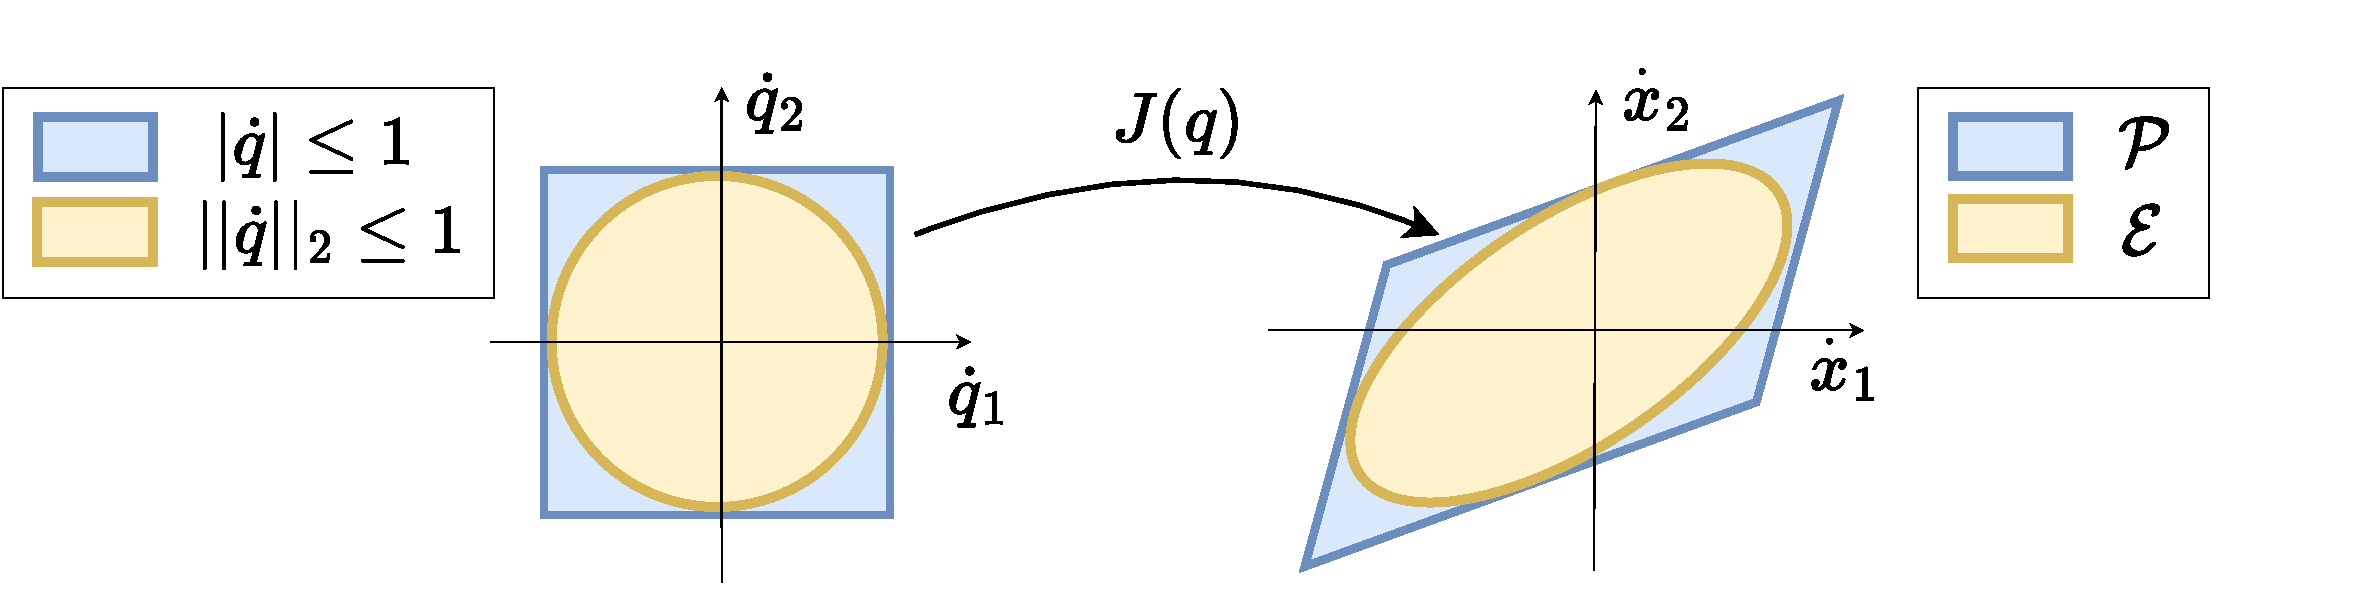
\includegraphics[width=0.8\textwidth]{Chapters/imgs/ellip_poly.pdf}
    \caption{An example manipulability polytope and ellipsoid geometry for a planar $m=2$ robot with $n=2$. The difference between the \gls{js} limits for ellipsoid described with $||\dot{\bm{q}}||_2\leq1$ (orange) and the range limits $\bm{-1}\leq\dot{\bm{q}}\leq\bm{1}$ (blue) is shown on the right. The difference in obtained achievable task-space velocity $\dot{{x}}$ polytope ${P}$ (blue) and ellipsoid ${E}$ (orange) is shown on the right plot. The plots show that both in joint and task-space the ellipsoid metric is an underestimation of the true robot's capacity.}
    \label{fig:ellip_poly_dif_revisit}
\end{figure}

To compare the ellipsoid and polytope metrics, the example of the manipulability ellipsoid and manipulability polytope can be used. 

The manipulability ellipsoid, proposed by \citet{yoshikawa_manipulability_1985}, is defined as the set of all achievable task-space velocities ${\dot{\bm{x}}}$ for a given robot configuration ${q}$ and joint velocity limits $-\bm{1} \leq {\dot{\bm{q}}}\leq \bm{1}$, and it can be expressed as
\begin{equation}\label{eq:manip_ellipsoid}
\mathcal{E} = \{ \dot{\bm{x}} ~|~ \dot{\bm{x}} = J({q})\dot{\bm{q}}, \quad ||\dot{\bm{q}}||_2 \leq \bm{1} \}
\end{equation}

The equivalent polytope representation of the manipulability ellipsoid is the manipulability polytope, which is defined as the set of all achievable task-space velocities ${\dot{\bm{x}}}$ for a given robot configuration ${q}$ and joint velocity limits $-1 \leq {\dot{\bm{q}}}\leq 1$, and it can be expressed as
\begin{equation}\label{eq:manip_polytope}
\mathcal{P} = \{ \dot{\bm{x}} ~|~ \dot{\bm{x}} = J({q})\dot{\bm{q}}, \quad -\bm{1} \leq \dot{\bm{q}} \leq \bm{1} \}
\end{equation}

Figure 1. illustrates the difference between the manipulability ellipsoid and polytope for a planar robot with two joints. The manipulability ellipsoid is an underestimation of the true robot's capacity, as it considers that the robot's velocity limits have the shape of a sphere, while in reality the robot's velocity limits $-\bm{1} \leq {\dot{\bm{q}}}\leq \bm{1}$ define a cube. The manipulability polytope is a more accurate representation of the robot's capacity, as it considers the true shape of the robot's velocity limits. 

More generally, polytope based representations of different physical abilities present the exact solution both for robots and for human musculoskeletal models, while ellipsoids present an approximation. 
Figure 2. shows the difference between the force ellipsoid and polytope \cite{chiacchio_evaluation_1996} for one configuration of the Franka Emika Panda robot.

Ellipsoids, however, are much more present in the literature, as their computation is much faster than the computation of polytopes. 

\subsection{Evaluating ellipsoids}

Evaluating ellipsoids is a computationally efficient task, as it can be done using the \gls{svd} \cite{yoshikawa1985manipulability}. Ellipsoids can be fully defined using their principal axis and principal axis lengths. Once they are known, the ellipsoid can be easily visualized and used for further analysis.

\codet{pycapacity} provides tools for evaluating several common ellipsoid metrics for robots and humans, such as velocity (manipulability), force and acceleration, and it provides a set of tools for their easy visualisation implemented in the module \codet{pycapacity.visual}. All the ellipsoid manipulation is implemented within the generic object \codet{Ellipsoid}, available as a part of \codet{pycapacity.objects} module

\subsection{Evaluating polytopes}
\label{sec:pycapacity_impelmented_polytopes}
As described more in detail in \Cref{ch:transformin_polytopes}, evaluating polytopes consists in finding either the minimal set of their vertices, $\repr{V}$-representation, or the minimal set of the half-planes defining their faces, $\repr{H}$-representation. The $\repr{V}$-representation is often used for visualisation purposes, while the $\repr{H}$-representation is often integrated in different optimization problems, as it can be represented as a set of linear inequalities.

However, finding the $\repr{V}$-representation or the $\repr{H}$-representation of a polytope is a computationally expensive task, relying on different vertex and facet enumeration algorithms \cite{fukuda2004frequently}. The computational complexity of these algorithms depends on the polytope formulation, the dimensionality of the input (number of robot's joints or human muscles) and output spaces (1D, 2D, 3D or 6D Cartesian space) and the complexity of the polytope geometry (number of vertices and faces). 

Therefore, polytope evaluation is often a bottleneck in the computation of different physical ability metrics, especially for human musculoskeletal models, which have a large number of degrees of freedom and a large number of muscles. Furthermore, due to the inherent complexity of the polytope evaluation algorithms, finding the appropriate algorithm for a given polytope formulation and dimension ablity of the input and output spaces is not a trivial task.


\codet{Pycapcity} package aims to provide a selection of algorithms for polytope evaluation, capable of evaluating common physical ability polytopes in an easy to use and efficient way.  These algorithms are implemented in Python and can be used as standalone tools as well. 
Additionally, \codet{pycapacity} implements several common polytope manipulation operations such as: 
\begin{itemize}
    \item Transforming polytope form $\repr{H}$ to  $\repr{V}$-representation
    \item Transforming polytope form $\repr{V}$ to  $\repr{H}$-representation
    \item Triangulating the polytope's vertices (sometimes called face or $\repr{F}$-representation) 
    \item Creating polytope form the Convex-Hull of a point cloud
    \item Minkowski sum of polytopes, as described in \Cref{ch:operations_over_poly_stategies}
    \item Intersection of polytopes, as described in \Cref{ch:operations_over_poly_stategies}
    \item Chabyshev ball
\end{itemize}
All these operations are implemented within the generic class \codet{Polytope} and can be used to perform additional operations on any physical ability polytope of humans and robots. Moreover, this class and all the above operations can be used as a standalone library as well for the use-cases outside of the scope of physical ability polytopes. The \codet{Polytope} class and its functionalities can be accessed through the module \codet{pycapacity.objects}. Finally, the package provides tools for easy visualisation the 2D and 3D polytopes implemented in the module \codet{pycapacity.visual}.

\section{Implemented physical capacity metrics}

The package implements different physical ability metrics for robotic manipulators and humans based on musculoskeletal models.

\subsection{Robotic manipulators metrics}
\label{sec:pycapacity_robot}

For robotic manipulators the package implement several velocity, force and acceleration capacity calculation functions based on ellipsoids and polytopes. All the metrics are implemented within \codet{pycapacity.robot} module:

\begin{figure}[!h]
    \centering
    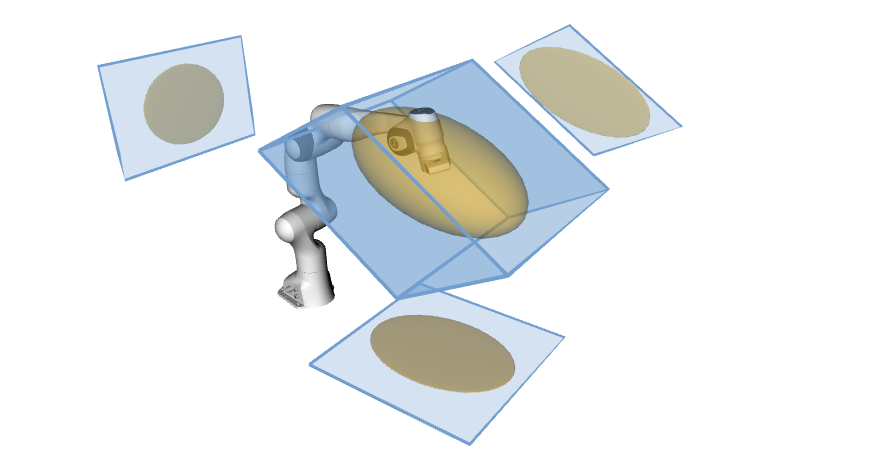
\includegraphics[width=0.7\linewidth]{Papers/images/polytope_ellipsoid.png}
    \caption{2D and 3D force polytopes and their ellipsoid counterparts for a 7 degrees of freedom (DOF) \textit{Franka Emika Panda} robot. Both polytopes and ellipsoids are calculated separately for the 3D and for each of the 2D reduced task-space cases. Both polytopes and ellipsoids take in consideration the true joint torque limits provided by the manufacturer. The underestimation of the true force capabilities of the robot by ellipsoids appears clearly}
    \label{fig:force_polytope_robot_ellip_revisit}
\end{figure}


\subsubsection*{Ellipsoids}
\begin{itemize}
\itemindent=-13pt
\item  Velocity (manipulability) ellipsoid, as described by \citet{yoshikawa_manipulability_1985} 
\begin{equation}\label{eq:ev_r}
\mathcal{E}_{v} = \{\dot{\bm{x}} ~| ~\dot{\bm{x}} = J\dot{\bm{q}},~ ||W^{-1}\dot{\bm{q}}||\leq1 \}, \qquad W = \text{diag}(\dot{\bm{q}}_{max})
\end{equation}
\item  Acceleration (dynamic manipulability) ellipsoid, as described by \citet{chiacchio_new_2000}
\begin{equation}\label{eq:ea_r}
\mathcal{E}_{a} = \{\ddot{\bm{x}} ~| ~\ddot{\bm{x}} = JM^{-1}\bm{\tau},~ ||W^{-1}\bm{\tau}||\leq1 \}, \qquad W = \text{diag}(\bm{\tau}_{max})
\end{equation}
\item  Force ellipsoid, as described by \citet{Chiacchio1997Force}
\begin{equation}\label{eq:ef_r}
\mathcal{E}_{f} = \{\bm{f} ~| ~J^{T}\bm{f} = \bm{\tau},~ ||W^{-1}\bm{\tau}||\leq1 \}, \qquad W = \text{diag}(\bm{\tau}_{max})
\end{equation}
\end{itemize}

Where $J$ is the robot's Jacobian matrix, $M$ is its mass matrix, $\bm{f}$ is the vector of \gls{cs} forces, $\dot{\bm{x}}$ and $\ddot{\bm{x}}$ are vectors of \gls{cs} velocities and accelerations, $\dot{\bm{q}}$ is the vector of the joint velocities and $\bm{\tau}$ is the vector of \gls{js} torques.

\subsubsection*{Polytopes}

\begin{itemize}
\itemindent=-13pt
\item Velocity polytope, described in \Cref{ch:vel_poly}
\begin{equation}\label{eq:pv_r}
\mathcal{P}_{v} = \{\dot{\bm{x}} ~| ~\dot{\bm{x}} = J\dot{\bm{q}},~ \dot{\bm{q}}_{min}\leq\dot{\bm{q}}\leq\dot{\bm{q}}_{max} \}
\end{equation}

\item Acceleration polytope, described in \Cref{ch:accel_poly_robot}
\begin{equation}\label{eq:pa_r}
\mathcal{P}_{a} = \{\ddot{\bm{x}} ~| ~\ddot{\bm{x}} = JM^{-1}\bm{\tau},~ \bm{\tau}_{min}\leq\bm{\tau}\leq\bm{\tau}_{max} \}
\end{equation}

\item Force polytope, described in \Cref{ch:poly_force}
\begin{equation}\label{eq:pf_r}
\mathcal{P}_{f} = \{\bm{f} ~| ~J^{T}\bm{f} = \bm{\tau},~ \bm{\tau}_{min}\leq\bm{\tau}\leq\bm{\tau}_{max} \}
\end{equation}

\item Minkowski sum and intersection of force polytopes
\begin{equation}\label{eq:psi_r}
\mathcal{P}_{\cap} = {P}_{f1} \cap {P}_{f1} \qquad P_{\oplus} = {P}_{f1} \oplus {P}_{f1} 
\end{equation}

\item Robot's reachable space approximation in the desired horizon of interest $\Delta t_{h}$ using the 
convex polytope formulation, described in \Cref{ch:hfr}
\begin{equation}\label{eq:prs_r}
\begin{split}
P_x = \{\Delta \bm{x}~ |~ \Delta \bm{x} &= JM^{-1}\bm{\tau} \frac{\Delta t_{h}^2}{2},\\
  {\bm{\tau}}_{min} &\leq \bm{\tau} \leq {\bm{\tau}}_{max},\\
   \dot{\bm{q}}_{min} &\leq M^{-1}\bm{\tau} \Delta t_{h}  \leq \dot{\bm{q}}_{max}, \\
  {q}_{min} &\leq M^{-1}\bm{\tau} \frac{\Delta t_{h}^2}{2}  \leq {q}_{max} \}\\
  \end{split}
\end{equation}
\end{itemize}

Where $J$ is the robot's Jacobian matrix, $M$ is its mass matrix, $\bm{f}$ is the vector of \gls{cs} forces, $\dot{\bm{x}}$ and $\ddot{\bm{x}}$ are vectors of \gls{cs} velocities and accelerations, $\dot{\bm{q}}$ is the vector of the joint velocities and $\bm{\tau}$ is the vector of \gls{js} torques.

\subsection{Human musculoskeletal model metrics}
\label{sec:pycapacity_human}

\begin{figure}[!h]
    \centering
    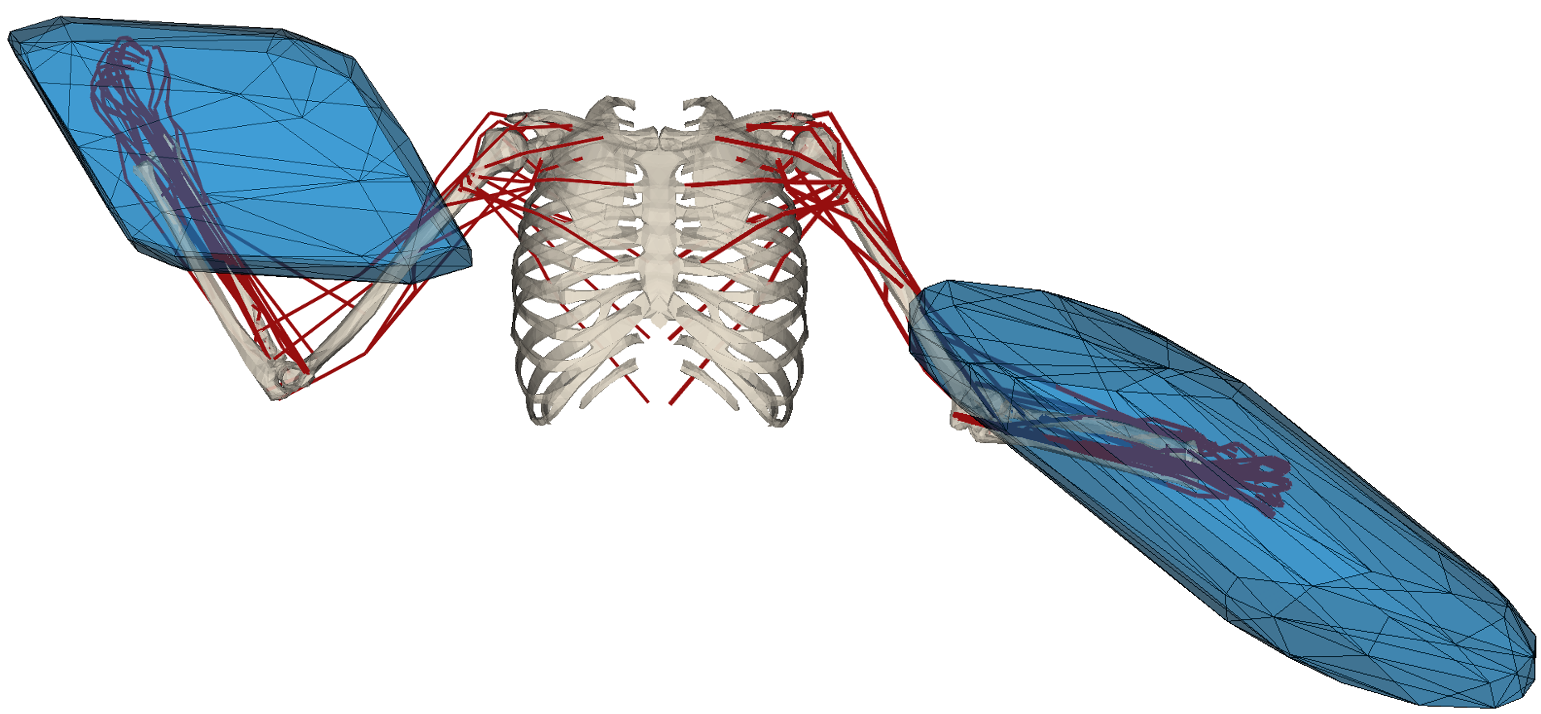
\includegraphics[width=0.7\linewidth]{Papers/images/bimanual.png}
    \caption{Cartesian force polytope of a musculoskeletal model of both human upper limbs with 7DOf and 50 muscles each, visualized with \codet{biorbd}. The polytopes are scaled with a ratio 1m : 1000N.}
    \label{fig:force_polytope_human_revisit}
\end{figure}

For the human musculoskeletal models this package implements the polytope and ellipsoid evaluation functions for the following metrics. All the metrics are implemented within \codet{pycapacity.human} module.

\subsubsection*{Ellipsoids}

\begin{itemize}
\itemindent=-13pt
\item Velocity (manipulability) ellipsoid, as described by \cite{yoshikawa_manipulability_1985}
\begin{equation}\label{eq:ev_dq_h}
\mathcal{E}_v = \{\dot{\bm{x}}~ |~ J\dot{\bm{q}} = \dot{\bm{x}}, \quad ||W^{-1}\dot{\bm{q}}|| \leq 1\}, \qquad W = \text{diag}(\dot{\bm{q}}_{max})
\end{equation}
\hspace{-13pt}
As well as its more complete formulation including muscular stretching velocities $\dot{\bm{l}}$
\begin{equation}\label{eq:ev_h}
\mathcal{E}_v = \{\dot{\bm{x}}~ |~ J\dot{\bm{q}} = \dot{\bm{x}},~ L\dot{\bm{q}} = \dot{\bm{l}} \quad ||W^{-1}\dot{\bm{l}}|| \leq 1\}, \qquad W = \text{diag}(\dot{\bm{l}}_{max})
\end{equation}

\item Acceleration (dynamic manipulability) ellipsoid, as proposed by \citet{khatib2009robotics}
\begin{equation}\label{eq:ea_r}
\mathcal{E}_{a} = \{\ddot{\bm{x}}~ |~ \ddot{\bm{x}} = JM^{-1}N\bm{F}, \quad ||W^{-1}\bm{F}|| \leq 1\}, \qquad W = \text{diag}(\bm{F}_{max})
\end{equation}

\item Force ellipsoid, as proposed by \citet{petric2019assistive}
\begin{equation}\label{eq:ef_r}
\mathcal{E}_{f} = \{\bm{f}~ |~ N\bm{F}  = J^T\bm{f},\quad ||W^{-1}\bm{F}|| \leq 1\}, \qquad W = \text{diag}(\bm{F}_{max})
\end{equation}
\end{itemize}
Where $J$ is the model's Jacobian matrix, $L$ is the muscle length Jacobian matrix, $N= -L^T$ is the moment arm matrix, $\bm{f}$ is the vector of \gls{cs} forces, $\dot{\bm{x}}$ and $\ddot{\bm{x}}$ are vectors of \gls{cs} velocities and accretions, $\dot{\bm{q}}$ is the vector of the \gls{js} velocities, $\bm{\tau}$ is the vector of \gls{js} torques, $\dot{\bm{l}}$ is the vector of the muscle stretching velocities and $\bm{F}$ is the vector of muscular forces. 

\subsubsection*{Polytopes}

\begin{itemize}
\itemindent=-13pt
\item Velocity polytope, described in \Cref{ch:human_vel_poly}
\begin{equation}\label{eq:pv_h}
\mathcal{P}_{v} = \{\dot{\bm{x}} ~|~\dot{\bm{l}} = L\dot{\bm{q}},~ \dot{\bm{x}} = J\dot{\bm{q}},~ \dot{\bm{q}}_{min}, ~ \leq\dot{\bm{q}}\leq\dot{\bm{q}}_{max}, ~\dot{\bm{l}}_{min}\leq\dot{\bm{l}}\leq\dot{\bm{l}}_{max} \}
\end{equation}

\item Acceleration polytope, described in \Cref{ch:human_aceleration_poly}  
\begin{equation}\label{eq:pa_h}
\mathcal{P}_{a} = \{\ddot{\bm{x}} ~|~ \ddot{\bm{x}} = JM^{-1}N\bm{F},~ \bm{F}_{min}\leq \bm{F}\leq \bm{F}_{max} \}
\end{equation}

\item Force polytope, described in \Cref{ch:force_poly_human}  
\begin{equation}\label{eq:pf_h}
\mathcal{P}_{f} = \{\bm{f} ~|~ J^T\bm{f} =N\bm{F},~ \bm{F}_{min}\leq \bm{F}\leq \bm{F}_{max} \}
\end{equation}
\end{itemize}

Where $J$ is the model's Jacobian matrix, $L$ is the muscle length Jacobian matrix, $N= -L^T$ is the moment arm matrix, $\bm{f}$ is the vector of \gls{cs} forces, $\dot{\bm{x}}$ and $\ddot{\bm{x}}$ are vectors of \gls{cs} velocities and accretions, $\dot{\bm{q}}$ is the vector of the \gls{js} velocities, $\bm{\tau}$ is the vector of \gls{js} torques, $\dot{\bm{l}}$ is the vector of the muscle stretching velocities and $\bm{F}$ is the vector of muscular forces. 

\section{Implemented polytope evaluation algorithms}
\label{sec:pycapacity_algos}

In addition to the efficient tools for generic polytope manipulation, listed in \Cref{sec:pycapacity_impelmented_polytopes}, the package implements several algorithms for polytope evaluation of the common formulations of physical ability polytopes of humans and robots

\begin{itemize}
    \item \gls{hpsm}
    \item Vertex Enumeration Algorithm (VEPOLI$^2$)
    \item Iterative Convex Hull Method (ICHM)
\end{itemize}

These algorithms are all implemented in Python and used to evaluate different polytope based physical ability metrics. Additionally, the algorithms are available to the users to be used standalone as well, and can be accessed through the module \codet{pycapacity.algorithms}.

\subsection{Hyper-plane shifting method (HPSM)}

This is an algorithm based on the article by \citet{hyper_psm} which presents an efficient way of determining the minimal half-space $\repr{H}$-representation of polytopes described by the equation 

\begin{equation}\label{eq:hpsm}
\mathcal{P} = \{ \bm{x} ~|~ \bm{x} = By, \quad y_{min}\leq y \leq y_{max} \}
\end{equation}

\subsection{Vertex enumeration algorithm (VEPOLI$^2$)}

This is an algorithm proposed in the context of this thesis, it is introduced in \Cref{sec:algorithm_vea}. This algorithm presents an efficient method for finding vertex $\repr{V}$-representation of polytopes described by the equation
\begin{equation}\label{eq:vertex_vepoli2}
\mathcal{P} = \{ \bm{x} ~|~ A\bm{x} = \bm{y}, \quad \bm{y}_{min}\leq \bm{y} \leq \bm{y}_{max} \}
\end{equation}


\subsection{Iterative convex-hull method (ICHM)}

This is an algorithm proposed in the context of this thesis as well, it is introduced in \Cref{ch:algorihtm_ichm}. This algorihtm implements an efficient method which iteratively approximates polytopes with a formulation
\begin{equation}\label{eq:ichm}
\mathcal{P} = \{ \bm{x} ~|~ A\bm{x} = B\bm{y}, \quad \bm{y}_{min}\leq \bm{y} \leq \bm{y}_{max} \}
\end{equation}

The method finds both vertex $\repr{V}$ and half-plane $\repr{H}$ representation of the polytope at the same time. The ICHM method implemented within the \codet{pycapacity} package can be additionally extended to the case where there is an additional projection matrix $P$ making a class of problems
\begin{equation}\label{eq:ichm_full}
\mathcal{P} = \{ \bm{x} ~|~ \bm{x}= P\bm{z}, ~A\bm{z} = B\bm{y}, \quad \bm{y}_{min}\leq \bm{y} \leq \bm{y}_{max} \}
\end{equation}


\section{Performance evaluation of polytope metrics}
\label{sec:pycapacity_performance}
As describe more in detail in \Cref{ch:transformin_polytopes}, the applicable methods to evaluate different polytope based physical abilities depend on the family of problems they correspond to. Therefore, this section brings the information about which algorithm is used for which polytope metric and provides a brief performance evaluation of their execution times.

Additionally, to give brief information about the efficiency of the proposed methods, the section provides the execution times of the methods for the example problems. However, as these execution times can vary significantly depending on the complexity of the model used and the hardware it is run on, the users are encouraged to run the benchmark scripts themselves to get the most accurate results. This package provides several benchmarking scripts in the \codet{examples} folder.

\subsection{Robotic manipulators}

In case of robotic manipulators the polytope evaluation methods used are given in \Cref{tab:methods_robots}.
\begin{table}[h]
\centering
\begin{tabular}{|l|l|l|l|}
\hline
Polytope Metric & Algorithm & Problem type & \makecell[c]{Execution time [ms] \\ mean $\pm$ std. (max)}  \\
\hline
Velocity & HPSM & $\bm{x}=B\bm{y},~ \bm{y} \in [\bm{y}_{min}, ~\bm{y}_{max}]$ & 3.6 $\pm$ 0.21 (5.7) \\
Acceleration & HPSM & $\bm{x}=B\bm{y},~ \bm{y} \in [\bm{y}_{min}, ~\bm{y}_{max}]$ & 6.6 $\pm$ 1.4 (14.2) \\
Force & VEPOLI$^2$ & $A\bm{x}=\bm{b}, ~\bm{b} \in [\bm{b}_{min}, ~\bm{b}_{max}]$ & 6.8 $\pm$ 0.88 (16.4) \\
Force intersection & VEPOLI$^2$ & $A\bm{x}=\bm{b},~\bm{b} \in [\bm{b}_{min}, ~\bm{b}_{max}]$ & 98.2 $\pm$ 29.33 (165.8) \\
Force sum & VEPOLI$^2$ & $A\bm{x}=\bm{b},~\bm{b} \in [\bm{b}_{min}, ~\bm{b}_{max}]$ & 17.1 $\pm$ 3.4 (44.9) \\
Reachable space & ICHM & $\bm{x}=B\bm{y},~ \bm{y} \in P_{y}$ & 30.5 $\pm$ 6.6 (76.7) \\
\hline
\end{tabular}
\caption{Performance evaluation of polytope metrics for robotic manipulators.}
\label{tab:methods_robots}
\end{table}

% Polytope Metric | Algorithm | Problem type | Execution time [ms] <br> mean $\pm$ std. (max)
% --- | -- | ----- | ----
% Velocity | HPSM | $\bm{x}=B\bm{y},~ \bm{y} \in [\bm{y}_{min}, ~\bm{y}_{max}]$ | 3.6 $\pm$ 0.21 (5.7)
% Acceleration |  HPSM | $\bm{x}=B\bm{y},~ \bm{y} \in [\bm{y}_{min}, ~\bm{y}_{max}]$ | 6.6 $\pm$ 1.4 (14.2)
% Force  | VEPOLI$^2$ | $A\bm{x}=\bm{b}, ~\bm{b} \in [\bm{b}_{min}, ~\bm{b}_{max}]$| 6.8 $\pm$ 0.88 (16.4)
% Force intersection |  VEPOLI$^2$ | $A\bm{x}=\bm{b},~\bm{b} \in [\bm{b}_{min}, ~\bm{b}_{max}]$ | 98.2 $\pm$ 29.33 (165.8)
% Force sum |  VEPOLI$^2$ | $A\bm{x}=\bm{b},~\bm{b} \in [\bm{b}_{min}, ~\bm{b}_{max}]$ | 17.1 $\pm$ 3.4 (44.9)
% Reachable space |  ICHM | $\bm{x}=B\bm{y},~  y \in P_{y}$ | 30.5 $\pm$ 6.6 (76.7)

The average execution time is calculated for 1000 random configuration of a 7 DOF Franka Emika panda robot, the model was used with \codet{pinocchio} \cite{pinocchio2021} library. All the experiments are run on a computer equipped with a 1.90GHz Intel i7-8650U processor. The results are obtained using the benchmarking script provided in the by the repository in the \codet{examples} folder. 

\subsection{Musculoskeletal models}

In case of human musculoskeletal models the methods used are given in \Cref{tab:methods_humans}.
\begin{table}[h]
\centering
\begin{tabular}{|l|l|l|l|}
\hline
Polytope Metric & Algorithm & Problem type & \makecell[c]{Execution time [ms] \\ mean $\pm$ std. (max)} \\
\hline
Force & ICHM & $A\bm{x}=B\bm{y},~ \bm{y} \in [\bm{y}_{min}, ~\bm{y}_{max}]$ & 186.8 $\pm$ 45.6 (281.6) \\
Acceleration & HPSM or ICHM & $\bm{x}=B\bm{y},~ \bm{y} \in [\bm{y}_{min}, ~\bm{y}_{max}]$ & 378.8 $\pm$ 62.3 (643.7) \\
Velocity & ICHM & $\bm{x}=B\bm{y},~ \bm{y} \in P_{y}$ & 223.1 $\pm$ 60.4 (389.1) \\
\hline
\end{tabular}
\caption{Performance evaluation of polytope metrics for human musculoskeletal models.}
\label{tab:methods_humans}
\end{table}
% Polytope Metric  | Algorithm | Problem type | Execution time [ms] <br> mean $\pm$ std. (max)
% -- | --- | ----- | ----
% Force  | ICHM | $A\bm{x}=\bm{b}y,~ \bm{y} \in [\bm{y}_{min}, ~\bm{y}_{max}]$ | 186.8 $\pm$ 45.6 (281.6)
% Acceleration |  HPSM or ICHM | $x=By,~ \bm{y} \in [\bm{y}_{min}, ~\bm{y}_{max}]$ |  378.8 $\pm$ 62.3 (643.7)
% Velocity | ICHM | $x=By,~ y \in P_{y}$ | 223.1 $\pm$ 60.4 (389.1)

The average execution time is calculated for 1000 random configuration of a 50 muscle 7 DOF musculoskeletal model described by \citet{holzbaur2005model}, the model was used with \codet{biorbd} \cite{Michaud2021} biomechanics library. The experiments are run on a computer equipped with a 1.90GHz Intel i7-8650U processor. The results are obtained using the benchmarking script provided in the by the repository in the \codet{examples} folder. 

\qrimg{qrcodes/pycapacity.png}{https://auctus-team.github.io/pycapacity/}{\codet{pycapacity}}
\section{Package overview}
\label{sec:pycapacity_package_overview}
Python package \codet{pycapacity} is publicly available both as a GitHub repository\footnote{GitHub repo: \url{https://github.com/auctus-team/pycapacity}} and as a \codet{pip} package\footnote{\codet{pip} package: \url{https://pypi.org/project/pycapacity/}}. Furthermore, the package has up-to-date and comprehensive documentation\footnote{Documentation: \url{https://auctus-team.github.io/pycapacity/}} including many examples, showing both the package's functionalities and how to integrate it with other libraries. 

Installing the package can be done using a single line of code, using \codet{pip} package manager 
\begin{minted}{bash}
> pip install pycapacity
\end{minted}

\subsubsection*{Package structure}
The package is divided in 6 modules which can be used as standalone tools as well
\begin{itemize}
    \item \codet{pycapacity.objects} - Module implementing generic \texttt{Polytope} and \texttt{Ellipsoid} classes 
    \item \codet{pycapacity.algorihtms} - Polytope evaluation algorithms described in \Cref{sec:pycapacity_algos} 
    \item \codet{pycapacity.human} - Physical ability metrics for humans described in \Cref{sec:pycapacity_human}
    \item \codet{pycapacity.robot} - Physical ability metrics for robots described in \Cref{sec:pycapacity_robot}
    \item \codet{pycapacity.visual} - 2D and 3D visualisation of polytopes and ellipsoids
    \item \codet{pycapacity.examples} - Module implementing different toy models for fast prototyping
\end{itemize}



\subsubsection*{Example code}
To demonstrate the user-friendly nature of \codet{pycpacity}, this section provides an illustrative example involving the computation of a \gls{cs} force for a $m=3$ polytope $\mathcal{P}_f$. This polytope is associated with a randomised robot manipulator featuring $n=6$ degrees of freedom.  Furthermore, the obtained polytope $\mathcal{P}_f$ is intersected with a generic cube $\mathcal{C}_f$ and visualised. The resulting program output is displayed in \Cref{fig:pycapacity_example} for reference.
{\begin{wrapfigure}{r}{0.5\linewidth}
\vspace{7.5cm}
    \centering
    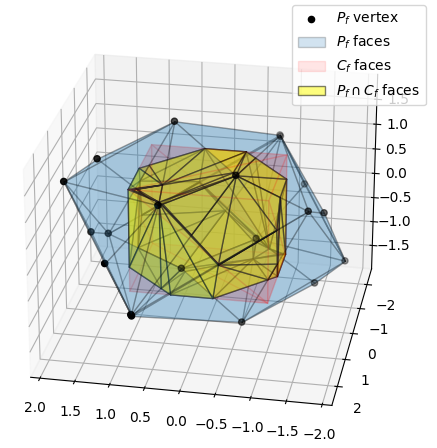
\includegraphics[width=\linewidth]{Papers/images/polytope_example.png}
    \caption{Output of the example program.}
    \label{fig:pycapacity_example}
\end{wrapfigure}

\begin{minted}[fontsize=\footnotesize, linenos]{python}
# robot capacity module
from pycapacity import robot, visual, objects
import matplotlib.pyplot as plt
import numpy as np

# radomised robot data
m, n = 3, 6 # 3d forces, 6 dof 
# joint torque limits max and min
t_min, t_max = -np.ones(n), np.ones(n) 
# random jacobian matrix
J = np.array(np.random.rand(m,n))*2-1

# calculate the force polytope
P_f = robot.force_polytope(J, t_min, t_max) 

# define a cube with H-representation
I = np.eye(3)
C_f = objects.Polytope(H = np.vstack((I,-I)), 
                       d = np.ones(6))  
# calculate the intersection
P_int = P_f & C_f
                    
# plotting the polytope
visual.plot_polytope(plot=plt, 
                    polytope=P_f, 
                    label='$P_f$',
                    edge_color='black',
                    alpha=0.2)
# plotting the cube
visual.plot_polytope(plot=plt, 
                    polytope=C_f,  
                    label='$C_f$',
                    color='red',
                    alpha=0.1)
# plotting the intersection
visual.plot_polytope(plot=plt, 
                    polytope=P_int, 
                    label='$P_f\cap C_f$',
                    color='yellow',
                    alpha=0.5)
plt.legend()
plt.show()
\end{minted}
}


\section{Conclusion}

This chapter introduces the \codet{pycapacity} Python package, a toolkit designed to evaluate task-space physical ability metrics for both humans and robots based on polytopes and ellipsoids. The aim of this package is to provide efficient tools for evaluating these metrics within an easily accessible framework, which can seamlessly integrate with standard robotics and biomechanics libraries. By implementing state-of-the-art algorithms for polytope evaluation, \codet{pycapacity} enables the evaluation of these metrics in an efficient manner, making them applicable for interactive online applications.